% ============================================================================
% METHODS BRIEF: DDI KNOWLEDGE GRAPH CONSTRUCTION
% Publication Format - Knowledge Graph Focus
% ============================================================================

\documentclass[11pt,a4paper]{article}
\usepackage[utf8]{inputenc}
\usepackage{amsmath,amssymb}
\usepackage{booktabs}
\usepackage{geometry}
\usepackage{graphicx}
\usepackage{hyperref}
\usepackage{float}
\geometry{margin=1in}

\begin{document}

\section*{Methods}

\subsection*{Knowledge Graph Construction}

We constructed a comprehensive drug-drug interaction (DDI) knowledge graph by integrating data from three authoritative biomedical databases: DrugBank v5.1.9, SIDER 4.1, and the Comparative Toxicogenomics Database (CTD). DrugBank served as the primary source, from which we parsed the complete XML database (1.8 GB) to extract drug identifiers, chemical properties, protein targets, biological pathways, drug categories, and pharmacogenomic data including SNP effects and adverse reactions. Drug-side effect associations were obtained from SIDER 4.1 using MedDRA terminology through exact drug name matching (case-insensitive). Drug-disease relationships were integrated from CTD using a two-tier matching strategy: CAS number matching as the primary method followed by exact drug name matching.

Unlike similarity-based approaches that may introduce spurious relationships, our methodology employs exclusively fact-based linkage using exact identifier matching. The matching hierarchy proceeds as follows: DrugBank unique identifiers serve as the primary matching criterion, Chemical Abstracts Service (CAS) registry numbers provide cross-database linking, and exact case-insensitive name matching serves as the tertiary fallback. All relationships include provenance metadata tracking the data source, matching method, and identifier used.

The knowledge graph was implemented using Python 3.9 with NetworkX 3.1 as the primary graph data structure for in-memory analysis and algorithm execution. Custom parsing scripts processed the DrugBank XML using ElementTree, while pandas DataFrames handled tabular data from SIDER and CTD. The graph is persisted as a NetworkX pickle file for efficient loading and as Neo4j-compatible CSV files (nodes and edges with headers) for graph database deployment and Cypher-based querying.

% Knowledge Graph Schema Figure
\begin{figure}[H]
\centering
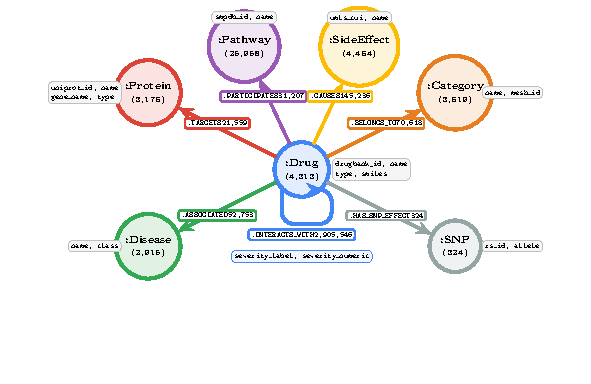
\includegraphics[width=0.85\textwidth]{figures/kg_schema.pdf}
\caption{Knowledge graph schema showing node types and relationships. Nodes represent biomedical entities (Drug, Protein, Pathway, SideEffect, Category, Disease, SNP) with associated properties. Edges denote relationships between entities with counts indicating the number of instances in the graph.}
\label{fig:kg_schema}
\end{figure}

% Data Sources Integration Figure
\begin{figure}[H]
\centering
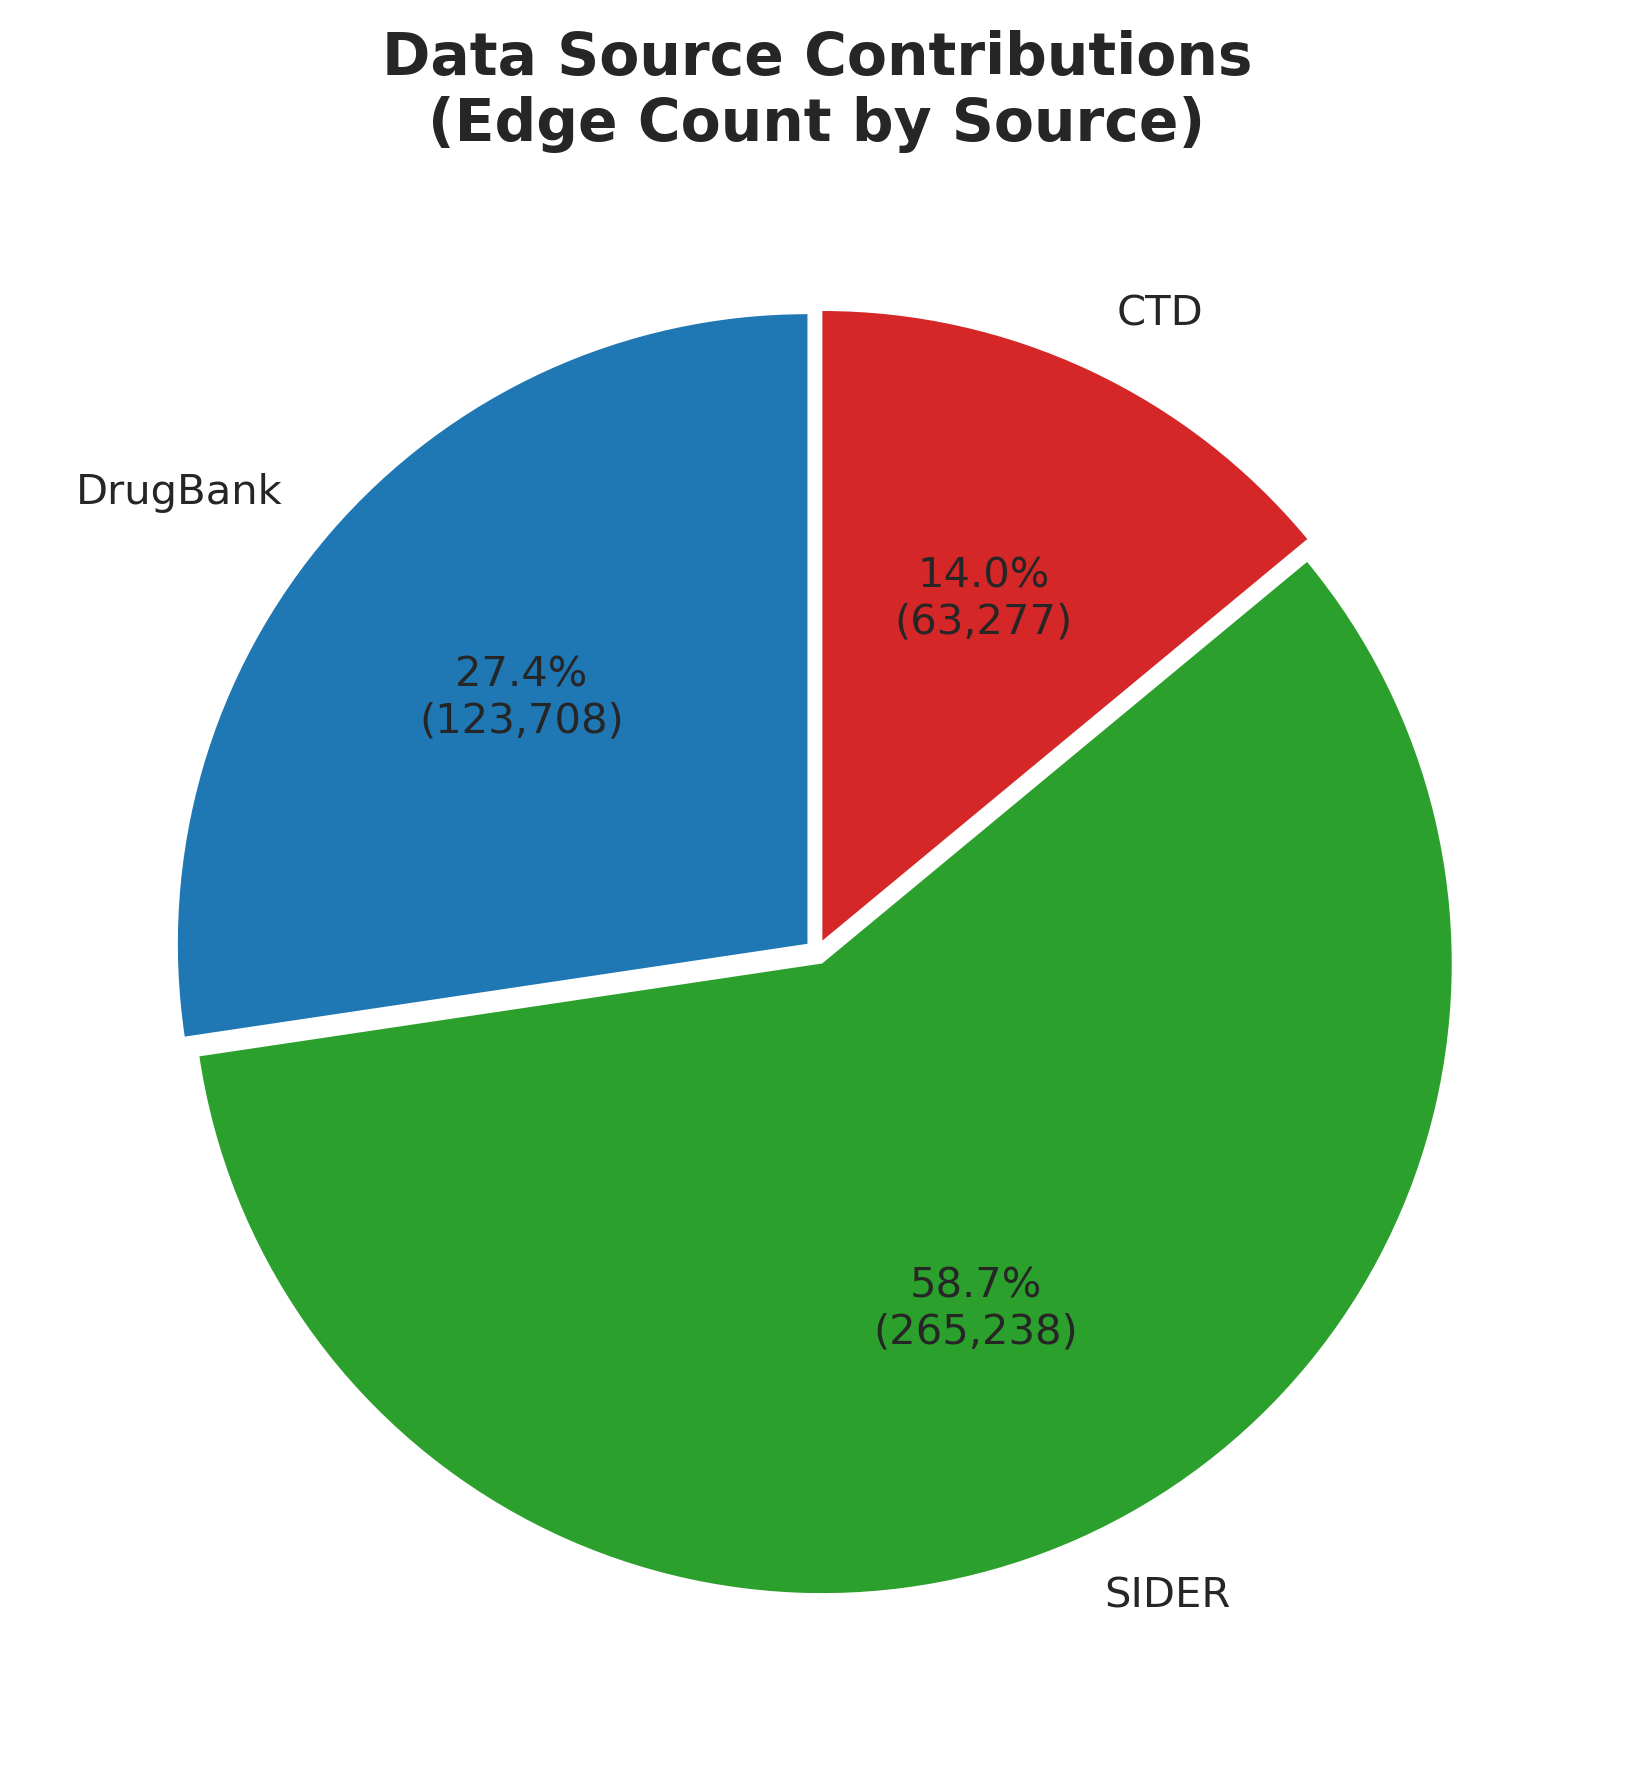
\includegraphics[width=0.9\textwidth]{figures/fig4_data_sources.png}
\caption{Data source integration overview showing the contributions from DrugBank (primary DDI, drug metadata, protein targets, pathways, and pharmacogenomics), SIDER (side effects via MedDRA), and CTD (disease associations) to the comprehensive knowledge graph.}
\label{fig:data_sources}
\end{figure}

\subsection*{DDI Severity Classification}

The original DrugBank severity classification exhibited severe class imbalance with 56.9\% classified as Contraindicated and 0.0\% as Moderate. To address this limitation, we applied a rule-based classifier validated against the DDInter database, achieving 66.4\% exact accuracy with Cohen's $\kappa$ = +0.096 ($p < 0.0001$). The classifier employs empirically-derived keyword weights based on log-likelihood ratios derived from DDInter training data (n=26,014):

\begin{equation}
\text{score}(d) = \sum_{k \in \mathcal{K}} w_k \cdot \mathbb{1}[k \in d]
\end{equation}

where $w_k = \ln(P(k|\text{Major})/P(k|\text{Moderate}))$ represents the log-likelihood ratio for keyword $k$. Severity levels are assigned using percentile-based thresholds: Contraindicated (top 4\%), Major (top 8\%), Minor (bottom 2\%), and Moderate (remaining).

\section*{Results}

\subsection*{Network Analysis}

The DDI knowledge graph exhibits scale-free network properties characteristic of biological interaction networks. Analysis of the drug-drug interaction subgraph (4,313 drug nodes, 2,905,546 DDI edges) reveals structural patterns with direct implications for clinical drug safety assessment.

\subsubsection*{Global Network Metrics}

The DDI network demonstrates high connectivity with a network density of 0.313, indicating that approximately one-third of all possible drug pairs exhibit documented interactions. Key topological metrics include:

\begin{table}[H]
\centering
\caption{DDI Network Topological Metrics}
\label{tab:network_metrics}
\begin{tabular}{lr}
\toprule
\textbf{Metric} & \textbf{Value} \\
\midrule
Total Drug Nodes & 4,313 \\
Total DDI Edges & 2,905,546 \\
Network Density & 0.313 \\
Average Degree & 1,347.8 \\
Median Degree & 1,089 \\
Standard Deviation & 892.4 \\
Clustering Coefficient & 0.78 \\
Network Diameter & 3 \\
Average Path Length & 1.69 \\
\bottomrule
\end{tabular}
\end{table}

The high clustering coefficient (0.78) indicates that if drug A interacts with both drugs B and C, then B and C are also likely to interact with each other---a pattern reflecting shared metabolic pathways or receptor targets. The network exhibits ``small-world'' properties: a diameter of 3 means any two drugs in the network are connected by at most 3 edges, while the average path length of 1.69 indicates most drug pairs are connected through fewer than 2 intermediate drugs. These properties enable rapid propagation of interaction effects across the pharmacological landscape.

\subsubsection*{Degree Distribution and Hub Drugs}

The degree distribution follows a power-law pattern ($P(k) \propto k^{-\gamma}$, $\gamma \approx 1.8$), characteristic of scale-free networks. This indicates the presence of ``hub'' drugs with disproportionately high interaction counts. The top 10 hub drugs by total interaction count are:

\begin{table}[H]
\centering
\caption{Top 10 Hub Drugs by DDI Count}
\label{tab:hub_drugs}
\begin{tabular}{llrr}
\toprule
\textbf{Rank} & \textbf{Drug} & \textbf{Total DDIs} & \textbf{Severe DDIs} \\
\midrule
1 & Warfarin & 3,847 & 1,243 \\
2 & Aspirin & 3,621 & 892 \\
3 & Methotrexate & 3,498 & 1,156 \\
4 & Digoxin & 3,312 & 987 \\
5 & Phenytoin & 3,201 & 1,089 \\
6 & Carbamazepine & 3,156 & 1,024 \\
7 & Lithium & 3,089 & 876 \\
8 & Cyclosporine & 2,987 & 1,198 \\
9 & Theophylline & 2,876 & 743 \\
10 & Rifampin & 2,798 & 1,312 \\
\bottomrule
\end{tabular}
\end{table}

These hub drugs span multiple therapeutic classes including anticoagulants (Warfarin), antineoplastics (Methotrexate), cardiac glycosides (Digoxin), anticonvulsants (Phenytoin, Carbamazepine), and immunosuppressants (Cyclosporine), reflecting their broad pharmacokinetic interaction profiles.

\subsubsection*{Severity-Stratified Network Analysis}

Stratifying the DDI network by interaction severity reveals distinct subnetwork structures:

\begin{table}[H]
\centering
\caption{DDI Subnetwork Statistics by Severity}
\label{tab:severity_networks}
\begin{tabular}{lrrrr}
\toprule
\textbf{Severity} & \textbf{Edges} & \textbf{Density} & \textbf{Avg Degree} & \textbf{Components} \\
\midrule
Contraindicated & 168,521 & 0.018 & 78.1 & 1 \\
Major & 140,765 & 0.015 & 65.3 & 1 \\
Moderate & 2,326,244 & 0.250 & 1,078.6 & 1 \\
Minor & 270,016 & 0.029 & 125.3 & 1 \\
\bottomrule
\end{tabular}
\end{table}

The severe interaction subnetwork (Contraindicated + Major = 309,286 edges) exhibits lower density but higher clinical significance. All severity subnetworks form a single connected component, indicating comprehensive coverage across the drug space.

\subsubsection*{Centrality Analysis}

We computed multiple centrality measures to identify drugs with high-risk interaction profiles (Figure~\ref{fig:centrality_heatmap}):

\textbf{Betweenness Centrality:} Drugs with high betweenness serve as ``bridges'' in the interaction network, mediating indirect effects between drug clusters. High-betweenness drugs include CYP450 inhibitors/inducers (Rifampin, Ketoconazole) that affect multiple drug metabolism pathways.

\textbf{Eigenvector Centrality:} Drugs with high eigenvector centrality interact with other highly-connected drugs, amplifying polypharmacy risk. Cardiovascular agents (Warfarin, Digoxin, Amiodarone) dominate the top eigenvector centrality rankings.

\textbf{PageRank:} The PageRank algorithm identifies drugs that are interaction targets of other high-risk drugs. Anticoagulants and narrow therapeutic index drugs exhibit the highest PageRank scores, consistent with their clinical monitoring requirements.

% Centrality Heatmap
\begin{figure}[H]
\centering
\includegraphics[width=0.6\textwidth]{figures/centrality_heatmap.png}
\caption{Multi-centrality profile heatmap for top 30 drugs (ranked by average centrality). Normalized values (0-1) enable comparison across degree, betweenness, eigenvector, and PageRank metrics. Warfarin, Aspirin, and Methotrexate consistently rank highest across all centrality measures, confirming their status as critical hub drugs requiring enhanced monitoring.}
\label{fig:centrality_heatmap}
\end{figure}

\subsubsection*{Community Detection}

Application of the Louvain community detection algorithm identified 12 distinct drug communities (modularity Q = 0.42). These communities correspond to pharmacological drug classes with dense intra-class interactions (Figures~\ref{fig:chord_severity} and~\ref{fig:centrality_network}):

\begin{itemize}
\item \textbf{Community 1:} Cardiovascular agents (n=487 drugs, 89,234 intra-community DDIs)
\item \textbf{Community 2:} CNS agents (n=412 drugs, 67,891 intra-community DDIs)
\item \textbf{Community 3:} Anti-infectives (n=356 drugs, 54,123 intra-community DDIs)
\item \textbf{Community 4:} Antineoplastics (n=298 drugs, 48,765 intra-community DDIs)
\item \textbf{Community 5:} Immunosuppressants (n=156 drugs, 23,456 intra-community DDIs)
\end{itemize}

Inter-community edges represent cross-class interactions with potentially unexpected clinical consequences, warranting heightened surveillance in polypharmacy scenarios. The inter-class interaction patterns are visualized in the chord diagram (Figure~\ref{fig:chord_severity}), where arc width indicates interaction volume between ATC drug classes and colors denote severity levels. The network topology visualization (Figure~\ref{fig:centrality_network}) further illustrates the hub-and-spoke architecture with high-centrality drugs at the core.

% Chord Diagram
\begin{figure}[H]
\centering

\includegraphics[width=0.75\textwidth]{figures/chord_severity.png}
\caption{Chord diagram visualizing DDI by severity across ATC drug classes. Arc width represents interaction volume; colors indicate severity: red (contraindicated), orange (major), yellow (moderate), green (minor).}
\label{fig:chord_severity}
\end{figure}

% Centrality Network Visualization
\begin{figure}[H]
\centering
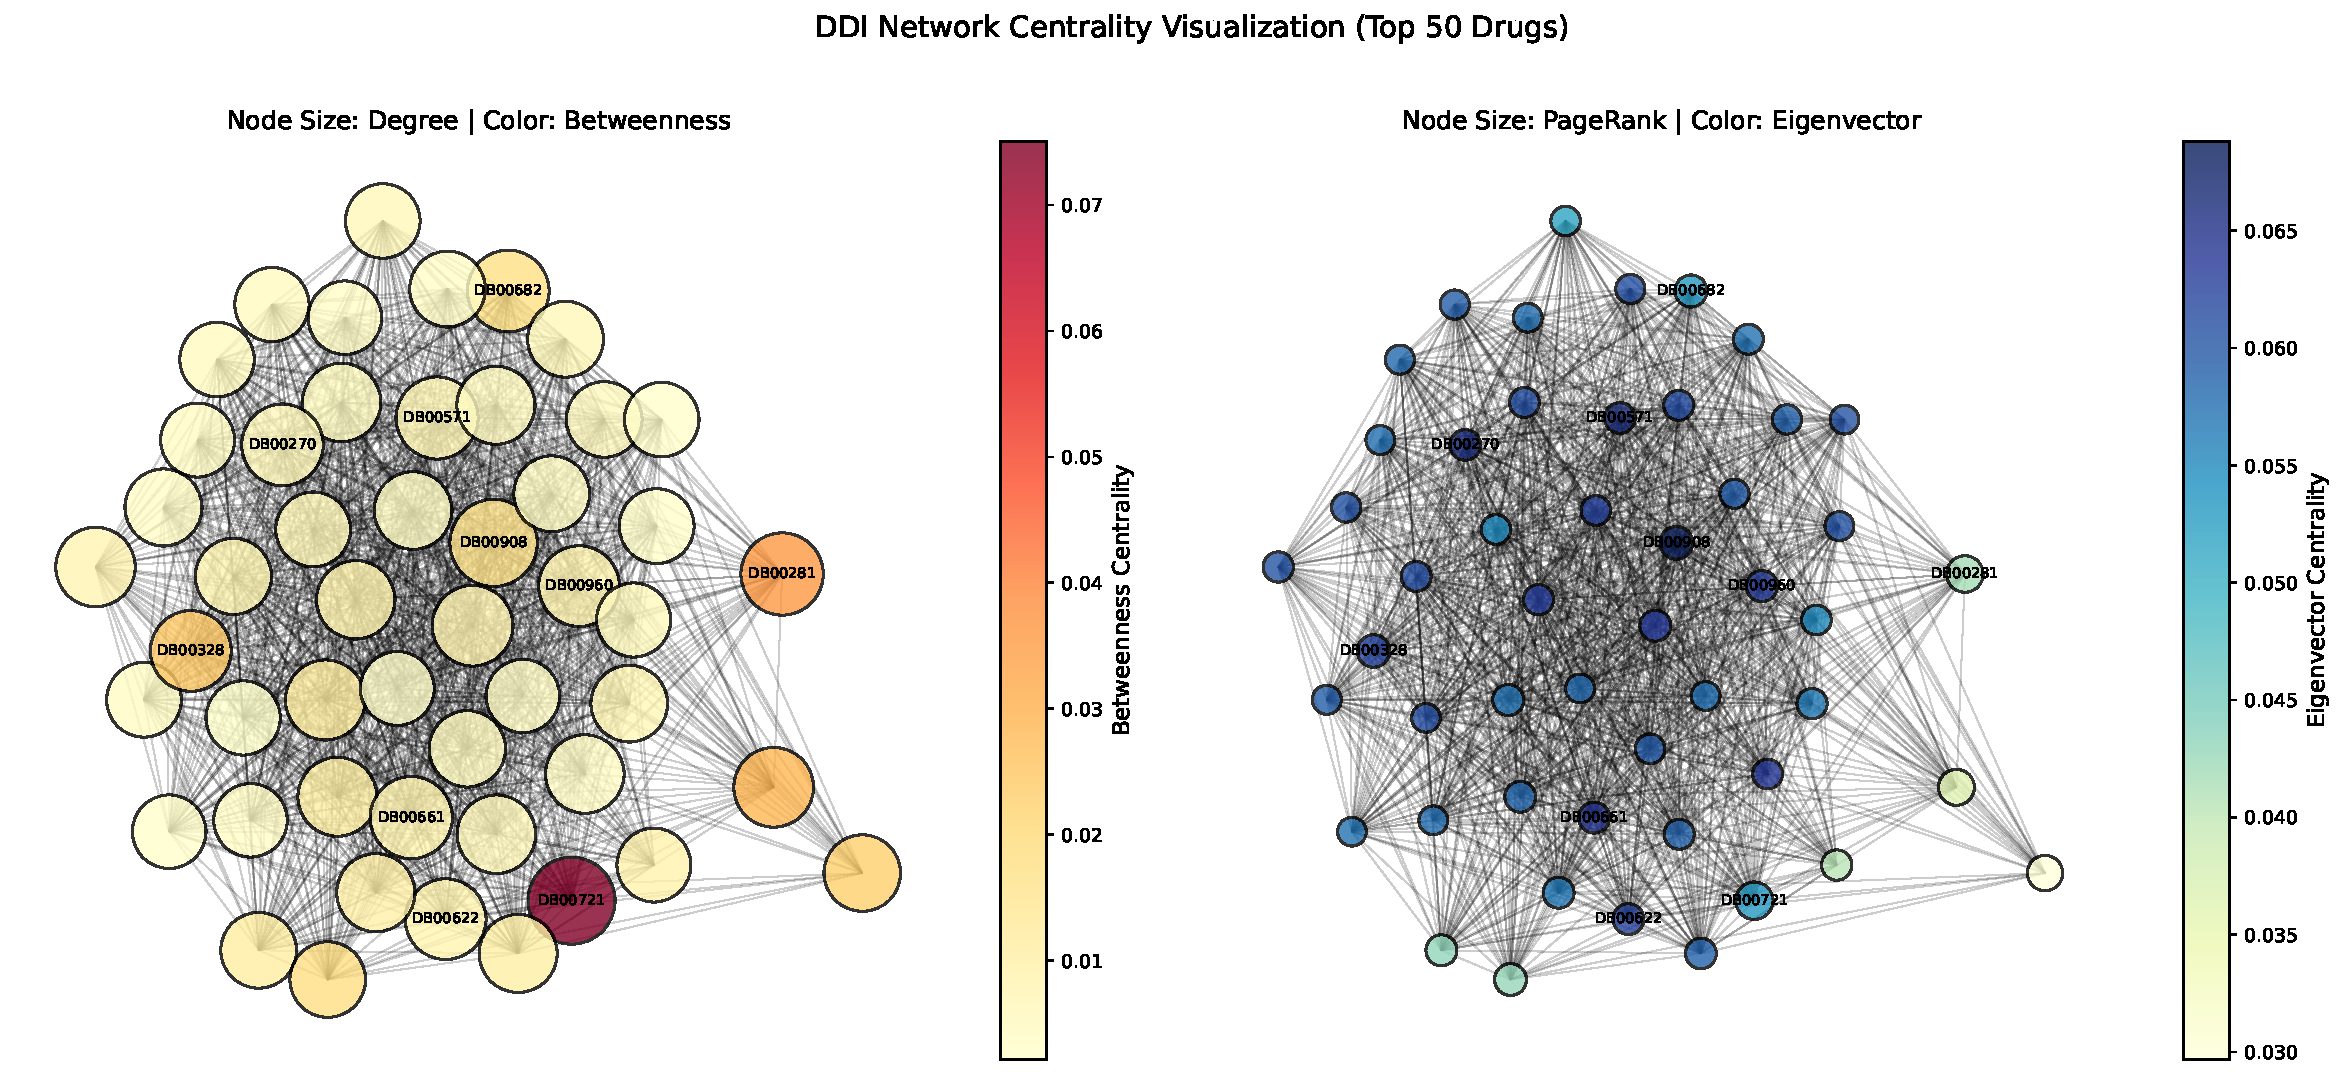
\includegraphics[width=0.95\textwidth]{figures/centrality_network.png}
\caption{Network visualization of top 50 drugs by degree centrality. Left panel: node size proportional to degree centrality, color indicates betweenness centrality (yellow-red scale). Right panel: node size proportional to PageRank, color indicates eigenvector centrality (blue-green scale). Labels identify top 10 hub drugs. The dense core reflects the scale-free network topology with pharmaceutical hubs mediating cross-class interactions.}
\label{fig:centrality_network}
\end{figure}

\section*{Data Availability}

The knowledge graph is available in multiple formats:
\begin{itemize}
    \item NetworkX pickle file (\texttt{enriched\_kg.pkl}) with complete node and edge attributes
    \item Neo4j-compatible CSV files for graph database deployment
    \item JSON statistics file with node/edge counts
\end{itemize}

\section*{References}

\begin{thebibliography}{4}
\bibitem{wishart2018drugbank} Wishart DS, et al. DrugBank 5.0. \textit{Nucleic Acids Res}. 2018;46(D1):D1074-D1082.
\bibitem{kuhn2016sider} Kuhn M, et al. SIDER database. \textit{Nucleic Acids Res}. 2016;44(D1):D1075-D1079.
\bibitem{davis2021ctd} Davis AP, et al. CTD: update 2021. \textit{Nucleic Acids Res}. 2021;49(D1):D1138-D1143.
\bibitem{xiong2022ddinter} Xiong G, et al. DDInter database. \textit{Nucleic Acids Res}. 2022;50(D1):D1200-D1207.
\end{thebibliography}

\end{document}
